\documentclass[11pt,a4paper]{article}

% ==============================================================================
% PAKKER OG GRUNNLEGGENDE OPPSETT
% ==============================================================================
\usepackage[utf8]{inputenc}
\usepackage[T1]{fontenc}
\usepackage[norsk]{babel}
\usepackage{amsmath, amssymb, amsfonts, bm}
\usepackage{graphicx}
\usepackage{booktabs}
\usepackage{microtype}
\usepackage[margin=2.5cm]{geometry}
\usepackage{caption}
\usepackage{subcaption}
\usepackage{siunitx}
\usepackage{float}
\usepackage{fancyhdr}
\usepackage{lastpage}
\usepackage{xcolor}
\usepackage{listings}
\usepackage{hyperref}

% Oppsett for desimalskilletegn og enheter
\sisetup{
    output-decimal-marker = {,},
    separate-uncertainty = true,
    per-mode = symbol
}

% Farger for hyperlenker og kode
\definecolor{ntnublue}{RGB}{0, 80, 158}
\definecolor{linkblue}{RGB}{0, 45, 125}
\definecolor{codegray}{rgb}{0.5,0.5,0.5}
\definecolor{codegreen}{rgb}{0.13,0.55,0.13}
\definecolor{codeblue}{rgb}{0.0,0.2,0.6}
\definecolor{codebackground}{rgb}{0.97,0.97,0.98}

% Hyperref oppsett
\hypersetup{
    colorlinks = true,
    linkcolor = linkblue,
    citecolor = linkblue,
    urlcolor = linkblue,
    pdftitle = {Eksperimentell og numerisk analyse av rullende kule på krum bane},
    pdfauthor = {Gruppe 3, NTNU Fysikk}
}

% Listings oppsett for Python-kode
\lstset{
    backgroundcolor=\color{codebackground},
    basicstyle=\ttfamily\footnotesize,
    breakatwhitespace=false,
    breaklines=true,
    captionpos=b,
    commentstyle=\color{codegreen}\itshape,
    keepspaces=true,
    keywordstyle=\color{codeblue}\bfseries,
    numbers=left,
    numbersep=7pt,
    numberstyle=\tiny\color{codegray},
    showspaces=false,
    showstringspaces=false,
    showtabs=false,
    stringstyle=\color{red!60!black},
    tabsize=4,
    frame=single,
    rulecolor=\color{gray!30}
}

% Sidehode og sidefot (fancyhdr)
\pagestyle{fancy}
\fancyhf{}
\fancyhead[L]{\small TFY4106 / TFY4125: Rullende kule på krum bane}
\fancyhead[R]{\small Gruppe 3}
\fancyfoot[C]{\small Side \thepage\ av \pageref{LastPage}}
\renewcommand{\headrulewidth}{0.4pt}
\renewcommand{\footrulewidth}{0.4pt}

% Figur- og tabelloppsett
\captionsetup{font=small, labelfont=bf, margin=10pt}

% ==============================================================================
% DOKUMENTSTART
% ==============================================================================
\begin{document}

% ------------------------------------------------------------------------------
% FORSIDE
% ------------------------------------------------------------------------------
\begin{titlepage}
    \centering
    \vspace*{0.5cm}

    % NTNU Logo med fallback
    \IfFileExists{ntnu_logo.png}{%
        
\includegraphics[width=0.38\textwidth]{ntnu_logo.png}%
    }{%
        \begin{center}
            \textsc{\Large \textbf{NTNU}}\\[0.2cm]
            \textsf{\small Norges teknisk-naturvitenskapelige universitet}
        \end{center}
    }

    \vspace{2.5cm}

    {\huge \bfseries Eksperimentell og numerisk analyse av rullende kule på krum bane\par}
    \vspace{0.6cm}
    {\Large \textsf{Laboratorierapport i TFY4106 / TFY4125 Fysikk}\par}

    \vspace{1.2cm}
    \rule{0.75\textwidth}{0.8pt}\par
    \vspace{1.2cm}

    {\large \textbf{Gruppe 3:}\par}
    \vspace{0.3cm}
    {\large
    Adrian Andersen \quad Thomas Neegård \quad Håkon Asheim\\[0.2cm]
    Filip Gløckner \quad Hilmar Holmen-Løkke \quad Anna Hødnebø\par}

    \vfill

    {\large
    Institutt for fysikk\\
    Norges teknisk-naturvitenskapelige universitet (NTNU), Trondheim\par}
    \vspace{0.8cm}
    {\large Høst 2026\par}
    \vspace*{0.5cm}
\end{titlepage}

\thispagestyle{empty}
\newpage

% ------------------------------------------------------------------------------
% SAMMENDRAG (ABSTRACT)
% ------------------------------------------------------------------------------
\begin{abstract}
\noindent
I dette laboratorieforsøket er bevegelsen til en kompakt kule som ruller på en todimensjonal krum bane undersøkt gjennom en kombinasjon av numeriske beregninger og eksperimentell videoanalyse. Baneprofilen ble formet ved hjelp av åtte justerbare festeskruer og modellert numerisk med en naturlig kubisk splineinterpolasjon. Den teoretiske modellen forutsetter ren rulling uten dissipasjon av mekanisk energi, hvor gravitasjonspotensiell energi konverteres fullstendig til translatorisk og rotatorisk kinetisk energi.

Modellens numeriske tidsintegrasjon resulterte i en teoretisk rulletid på $t_{\text{teor}} = \SI{1,828}{\second}$ og en teoretisk sluttfart på $v_{\text{teor}} = \SI{1,242}{\meter\per\second}$ ved banens ende ($x = \SI{1,40}{\meter}$). Eksperimentelle data fra åtte uavhengige rulleforsøk, filmet ved \SI{60}{fps} og analysert i sporingsprogrammet Tracker, ga en gjennomsnittlig målt rulletid på $t_{\text{målt}} = \SI{2,277 \pm 0,022}{\second}$ (utvalgsstandardavvik $s_t = \SI{0,061}{\second}$) og en gjennomsnittlig målt sluttfart på $v_{\text{slutt}} = \SI{0,994 \pm 0,010}{\meter\per\second}$ (utvalgsstandardavvik $s_v = \SI{0,029}{\meter\per\second}$). Den målte rulletiden er dermed omtrent \SI{24,6}{\percent} lengre og sluttfarten \SI{20,0}{\percent} lavere enn den ideelle modellens prediksjoner.

Det totale frigjorte potensielle energibidraget fra starthøyde til slutthøyde var $\Delta E_{\text{pot}} = \SI{33,45}{\milli\joule}$. Ved å inkludere både translasjon og rotasjon ble det gjennomsnittlige mekaniske energitapet bestemt til $\overline{\Delta E} = \SI{11,98 \pm 0,45}{\milli\joule}$ ($s_{\Delta E} = \SI{1,26}{\milli\joule}$), noe som utgjør et relativt tap av mekanisk energi på \SI{35,8}{\percent}. Den dynamiske kraftanalysen viste et maksimalt krav til statisk friksjonskoeffisient på $\max |f/N| = 0{,}144$, noe som tilsier at ren rulling i hovedsak var oppfylt. Det observerte energitapet skyldes i all hovedsak rullemotstand (elastisk hysterese i plastskinnene forsterket av to-punkts linjekontakt) og i mindre grad mikroskopisk sluring i soner med stor krumning samt luftmotstand. Forsøket viser at den ideelle numeriske modellen gir en god kvalitativ beskrivelse av banedynamikken, men fungerer kvantitativt som en teoretisk øvre grense for bevegelsen.
\end{abstract}

\vspace{1.0cm}
\tableofcontents
\newpage

% ------------------------------------------------------------------------------
% 1. INNLEDNING
% ------------------------------------------------------------------------------
\section{Innledning}
Studiet av stive legemers bevegelse på krumme flater utgjør et klassisk og fundamentalt problem innen klassisk mekanikk. Når et rullende legeme som en kule beveger seg under påvirkning av tyngdekraften, vekselvirker potensiell energi, translatorisk kinetisk energi og rotatorisk kinetisk energi i et koblet dynamisk system. I elementære teoretiske modeller formuleres bevegelsen ofte under forutsetning om et konservativt system der mekanisk energi er strengt bevart og kontakten mellom legemet og underlaget tilfredsstiller ren rulling uten glidning ($v = r\omega$).

I reelle fysiske systemer vil imidlertid legemet erfare ulike motstandskrefter, inkludert rullemotstand grunnet deformasjon av kontaktflaten, mikroskopisk sluring ved store vinkelakselerasjoner, samt aerodynamisk luftmotstand. Formålet med dette laboratorieforsøket i emnene TFY4106/TFY4125 Fysikk ved NTNU er todelt:
\begin{enumerate}
    \item Å etablere en ideell numerisk modell i Python som beregner kulas kontinuerlige baneform ved kubisk splineinterpolasjon, og deretter utlede kulas hastighetsprofil $v(x)$, tidsforbruk $t(x)$, normalkraft $N(x)$, friksjonskraft $f(x)$ og friksjonsforhold $|f/N|(x)$ basert på ren rulling og energibevaring.
    \item Å gjennomføre systematiske eksperimentelle målinger ved høyoppløselig videoopptak (\SI{60}{fps}) og digital massesentersporing i programvaren Tracker, for deretter å sammenligne modellens teoretiske prediksjoner med reelle observasjoner over åtte uavhengige forsøk.
\end{enumerate}
Gjennom en komparativ analyse kvantifiseres avvikene i rulletid og sluttfart. Videre foretas en grundig statistisk usikkerhetsanalyse og en fysisk drøfting av de dissipative mekanismene som forårsaker det mekaniske energitapet under bevegelsen.

% ------------------------------------------------------------------------------
% 2. TEORI OG BEREGNINGSGRUNNLAG
% ------------------------------------------------------------------------------
\section{Teori og beregningsgrunnlag}

\subsection{Baneprofil og differensialgeometri}
Banens vertikale profil beskrives ved en funksjon $y(x)$, der $x$ er den horisontale posisjonen og $y$ er høyden over et valgt referansenivå. Banen er eksperimentelt definert av $M = 8$ diskrete festepunkter $(x_j, y_j)$ for $j = 0, 1, \dots, 7$, montert med et jevnt horisontalt intervall $\Delta x_{\text{skrue}} = \SI{200}{\milli\meter}$ over en total lengde på $L = \SI{1400}{\milli\meter}$.

For å oppnå en glatt og to ganger kontinuerlig deriverbar kurve $y(x) \in C^2[x_0, x_7]$, interpoleres punktene ved hjelp av en kubisk spline. Mellom hvert intervall $[x_j, x_{j+1}]$ beskrives kurven av et tredjegradspolynom:
\begin{equation}
    S_j(x) = a_j + b_j(x - x_j) + c_j(x - x_j)^2 + d_j(x - x_j)^3, \quad x \in [x_j, x_{j+1}].
    \label{eq:spline_def}
\end{equation}
Koeffisientene bestemmes ved krav om kontinuitet i funksjonsverdi samt første- og andrederiverte i de indre skruepunktene:
\begin{equation}
    S_{j-1}(x_j) = S_j(x_j), \quad S'_{j-1}(x_j) = S'_j(x_j), \quad S''_{j-1}(x_j) = S''_j(x_j).
\end{equation}
Ved banens endepunkter benyttes naturlige randbetingelser, som innebærer at krumningen settes lik null:
\begin{equation}
    y''(x_0) = 0 \quad \text{og} \quad y''(x_7) = 0.
\end{equation}

Fra baneprofilens deriverte kan banens geometriske helningsvinkel $\beta(x)$ i ethvert punkt bestemmes ved:
\begin{equation}
    \beta(x) = \arctan\left(y'(x)\right).
    \label{eq:beta}
\end{equation}
Banens krumning $\kappa(x)$ er definert ut fra banens banekoordinatbue og uttrykkes analytisk ved de kartesiske deriverte som:
\begin{equation}
    \kappa(x) = \frac{y''(x)}{\left(1 + \left(y'(x)\right)^2\right)^{3/2}}.
    \label{eq:kappa}
\end{equation}
Krumningsradiusen er gitt ved $R(x) = 1/|\kappa(x)|$. Dersom banens krumning er oppoverbøyd (dal) er $\kappa(x) > 0$, mens en nedoverbøyd kurve (topp) har $\kappa(x) < 0$.

\subsection{Ren rulling og mekanisk energibevaring}
Vi betrakter en homogen, kompakt kule med masse $m$ og ytre radius $r$. Treghetsmomentet om en akse gjennom kulas massesenter er gitt ved:
\begin{equation}
    I = c m r^2, \quad \text{hvor } c = \frac{2}{5}.
    \label{eq:moment_inertia}
\end{equation}
Betingelsen for ren rulling (rulling uten glidning eller sluring) krever at kulas translatoriske banefart $v$ og vinkelhastighet $\omega$ er entydig koblet gjennom:
\begin{equation}
    v = r\omega.
    \label{eq:pure_rolling}
\end{equation}
Kulas totale kinetiske energi $K$ er summen av translatorisk bevegelsesenergi $K_{\text{trans}}$ og rotatorisk bevegelsesenergi $K_{\text{rot}}$:
\begin{equation}
    K = K_{\text{trans}} + K_{\text{rot}} = \frac{1}{2}mv^2 + \frac{1}{2}I\omega^2 = \frac{1}{2}mv^2 + \frac{1}{2}\left(c m r^2\right)\left(\frac{v}{r}\right)^2 = \frac{1}{2}(1 + c)mv^2.
\end{equation}
Ved å sette inn $c = 2/5$ for en kompakt kule, reduseres dette til:
\begin{equation}
    K = \frac{7}{10}mv^2.
    \label{eq:kin_energy}
\end{equation}
Under forutsetning om at dissipative krefter kan neglisjeres, er den totale mekaniske energien $E = U + K$ konstant langs hele banen:
\begin{equation}
    E(x) = mgy(x) + \frac{1}{2}(1 + c)mv(x)^2 = \text{konstant}.
\end{equation}
Når kula slippes fra ro ved starthøyden $y_0 = y(x_0)$ med startfart $v(x_0) = 0$, etablerer energibevaringen sammenhengen:
\begin{equation}
    mgy_0 = mgy(x) + \frac{1}{2}(1 + c)mv(x)^2.
\end{equation}
Løst med hensyn på kulas momentane banefart $v(x)$ gir dette:
\begin{equation}
    v(x) = \sqrt{\frac{2g\left(y_0 - y(x)\right)}{1 + c}} = \sqrt{\frac{10}{7}g\left(y_0 - y(x)\right)}.
    \label{eq:v_teor}
\end{equation}
Ligning~\eqref{eq:v_teor} viser at farten til ethvert tidspunkt utelukkende er bestemt av det vertikale fallet $y_0 - y(x)$ og treghetsmomentfaktoren $c$, uavhengig av kulas masse og radius.

\subsection{Tidsintegrasjon og numerisk beregning av rulletid}
Den horisontale hastighetskomponenten til massesenteret er gitt ved geometrisk projeksjon:
\begin{equation}
    v_x(x) = v(x)\cos\beta(x).
    \label{eq:vx}
\end{equation}
Fra definisjonen av hastighet $v_x = \mathrm{d}x/\mathrm{d}t$ følger det infinitesimale tidssteget:
\begin{equation}
    \mathrm{d}t = \frac{\mathrm{d}x}{v_x(x)} = \frac{\mathrm{d}x}{v(x)\cos\beta(x)}.
\end{equation}
Den totale teoretiske rulletiden $T$ fra startpunktet $x_0$ til sluttpunktet $x_f$ er gitt ved det bestemte integralet:
\begin{equation}
    T = \int_{x_0}^{x_f} \frac{\mathrm{d}x}{v(x)\cos\beta(x)}.
    \label{eq:tid_integral}
\end{equation}
I den numeriske koden beregnes dette integralet ved å diskretisere banen i $n = 1400$ delintervaller med steglengde $\Delta x = \SI{0,001}{\meter}$. Tidsbruken over hvert intervall tilnærmes ved trapesformelen basert på gjennomsnittlig horisontalhastighet:
\begin{equation}
    \Delta t_i \approx \frac{2\Delta x}{v_{x, i-1} + v_{x, i}}, \quad \text{for } i = 2, 3, \dots, n.
    \label{eq:trapezoid}
\end{equation}
I det aller første intervallet $[x_0, x_1]$ er startfarten $v_{x, 0} = 0$. For å unngå singularitet i nevneren antas konstant akselerasjon over dette første millimetersteget, hvilket gir:
\begin{equation}
    \Delta t_1 = \frac{2\Delta x}{v_{x, 1}}.
    \label{eq:dt_first}
\end{equation}
Kulas kumulative tidsprofil finnes deretter ved numerisk summasjon: $t(x_k) = \sum_{i=1}^k \Delta t_i$.

\subsection{Dynamiske kontaktkrefter og betingelse for ren rulling}
For å undersøke bevegelsens fysikk i detalj må kreftene i kontaktpunktet mellom kula og banen utledes. Vi dekomponerer Newtons 2.~lov i komponenter henholdsvis normalt på og parallelt med tangenten til banen.

\paragraph{Normalkraft og sentripetalakselerasjon:}
I normalretningen virker normalkraften $N(x)$ vinkelrett ut fra underlaget mot kulas massesenter, motvirket av tyngdekraftens normalkomponent $mg\cos\beta(x)$. Kulas normalakselerasjon (sentripetalakselerasjon) er gitt ved $a_n(x) = v(x)^2\kappa(x)$, der $\kappa(x)$ er banens fortegnsbestemte krumning. Newtons 2.~lov i normalretningen gir:
\begin{equation}
    N(x) - mg\cos\beta(x) = m a_n(x) = m v(x)^2\kappa(x),
\end{equation}
hvilket gir normalkraften:
\begin{equation}
    N(x) = m\left(g\cos\beta(x) + v(x)^2\kappa(x)\right).
    \label{eq:normalkraft}
\end{equation}
Det fysiske fortegnet til $\kappa(x)$ spiller her en avgjørende rolle:
\begin{itemize}
    \item I daler (bunnpunkter) bøyer banen oppover ($\kappa > 0$). Kula må akselereres oppover, slik at sentripetalkraften adderes til tyngdekraftens normalkomponent. Normalkraften oppnår derfor sine maksimale verdier i bunnpunktene: $N > mg\cos\beta$.
    \item På bakketopper (høydedrag) bøyer banen nedover ($\kappa < 0$). Kula presses mot utsiden av kurven, hvilket reduserer trykket mot banen: $N < mg\cos\beta$. Dersom $N(x)$ skulle bli null eller negativ, ville kula miste kontakten og lette fra banen.
\end{itemize}

\paragraph{Friksjonskraft og rotasjonsakselerasjon:}
Langs banens tangent virker tyngdekraftens tangensialkomponent $mg\sin\beta(x)$ og den statiske friksjonskraften $f(x)$. Newtons 2.~lov for translasjon langs banen lyder:
\begin{equation}
    mg\sin\beta(x) + f(x) = m a_t(x),
    \label{eq:newton_tang}
\end{equation}
der $a_t(x)$ er banens tangentialakselerasjon. Rotasjonsdynamikken om massesenteret bestemmes av friksjonskraftens dreiemoment, da normalkraften og tyngdekraften angriper gjennom massesenteret og gir null dreiemoment:
\begin{equation}
    \tau = -f(x) r = I \alpha(x) = \left(c m r^2\right) \frac{a_t(x)}{r} = c m r a_t(x).
    \label{eq:torque}
\end{equation}
Dette gir den fundamentale sammenhengen $f(x) = -c m a_t(x)$. Ved å substituere dette inn i ligning~\eqref{eq:newton_tang} finner vi:
\begin{equation}
    mg\sin\beta(x) - c m a_t(x) = m a_t(x) \implies a_t(x) = \frac{g\sin\beta(x)}{1 + c}.
\end{equation}
Friksjonskraften uttrykkes dermed analytisk som:
\begin{equation}
    f(x) = -\frac{c}{1 + c}mg\sin\beta(x) = -\frac{2}{7}mg\sin\beta(x).
    \label{eq:friksjon}
\end{equation}

\paragraph{Fysisk tolkning av friksjonskraftens fortegn:}
I definisjonen av $\beta(x) = \arctan(y'(x))$ er vinkelen negativ ($\beta < 0$) når banen heller nedover i bevegelsesretningen. Dermed er $\sin\beta(x) < 0$. Innsatt i ligning~\eqref{eq:friksjon} gir dette en \emph{positiv} friksjonskraft ($f > 0$). Fysisk innebærer dette at friksjonskraften virker oppover bakken langs banen. Dette er helt nødvendig: Når kula ruller nedover en bakke, må den spinne opp for å tilfredsstille rullebetingelsen $v = r\omega$. En kraft rettet oppover bakken gir et dreiemoment med klokka som øker rotasjonshastigheten, samtidig som den reduserer translatorisk akselerasjon i forhold til friksjonsfri glidning. Motsatt, når banen går oppover ($\beta > 0 \implies \sin\beta > 0$), blir $f < 0$, noe som betyr at friksjonskraften virker forover/nedover for å bremse kulas rotasjonshastighet i takt med retardasjonen.

\paragraph{Sklibetingelse (kriterium for ren rulling):}
Statisk friksjon kan maksimalt yte en kraft begrenset av Coulomb-amontons lov:
\begin{equation}
    |f(x)| \le \mu_s N(x),
\end{equation}
der $\mu_s$ er den statiske friksjonskoeffisienten mellom kulas overflate og banen. Kriteriet for at ren rulling skal opprettholdes uten at kula begynner å slure (gli), er følgelig:
\begin{equation}
    \frac{|f(x)|}{N(x)} \le \mu_s \quad \forall x \in [x_0, x_f].
    \label{eq:sklikrav}
\end{equation}
Minste påkrevde statiske friksjonskoeffisient for banen er dermed gitt ved modellens maksimale friksjonsforhold:
\begin{equation}
    \mu_{s, \min} = \max_{x} \left( \frac{|f(x)|}{N(x)} \right).
    \label{eq:mu_min}
\end{equation}

\subsection{Eksperimentell energiberegning og mekanisk energitap}
I reelle eksperimenter er det mekaniske systemet ikke konservativt. Det utføres arbeid mot ikke-konservative krefter som rullemotstand, mikroskopisk glidning og luftmotstand. Det totale mekaniske energitapet $\Delta E$ defineres som differansen mellom systemets mekaniske energi ved start og slutt:
\begin{equation}
    \Delta E = E_{\text{start}} - E_{\text{slutt}}.
    \label{eq:energitap_def}
\end{equation}
Kula slippes fra ro ved startpunktet ($v_0 = 0$), slik at $E_{\text{start}} = mgy_0$. Ved banens ende ($x = \SI{1,40}{\meter}$) befinner kula seg i høyden $y_f = y(x_f)$ med målt sluttfart $v_f$. Total mekanisk energi ved slutt er summen av sluttpotensiell energi og sluttkinetisk energi (både translasjon og rotasjon under antakelse om ren rulling ved utgangen):
\begin{equation}
    E_{\text{slutt}} = mgy_f + K_{\text{tot}} = mgy_f + \frac{7}{10}mv_f^2.
\end{equation}
Dermed uttrykkes det mekaniske energitapet for hvert enkelt forsøk $i$ som:
\begin{equation}
    \Delta E_i = mg(y_0 - y_f) - \frac{7}{10}mv_{f, i}^2 = \Delta E_{\text{pot}} - K_{\text{tot}, i}.
    \label{eq:delta_e_i}
\end{equation}
Her representerer $\Delta E_{\text{pot}} = mg(y_0 - y_f)$ den totale potensielle energien som frigjøres mellom start- og sluttposisjonen. Det relative mekaniske energitapet uttrykkes i prosent som:
\begin{equation}
    \eta_{\text{tap}} = \frac{\overline{\Delta E}}{\Delta E_{\text{pot}}} \times 100\,\%.
    \label{eq:rel_tap}
\end{equation}

\subsection{Statistisk databehandling og usikkerhetsanalyse}
For å kvantifisere tilfeldige feil og måleusikkerhet gjennomføres en statistisk analyse av $n = 8$ uavhengige måleserier i samsvar med NTNUs retningslinjer for usikkerhetsanalyse~\cite{lilledahl2017}. For en målestørrelse $q \in \{t, v_f, \Delta E\}$ beregnes utvalgets aritmetiske gjennomsnitt $\bar{q}$ ved:
\begin{equation}
    \bar{q} = \frac{1}{n} \sum_{i=1}^n q_i.
    \label{eq:mean}
\end{equation}
Variasjonen og spredningen mellom de individuelle målingene kvantifiseres ved utvalgsstandardavviket $s_q$, beregnet med $n - 1$ frihetsgrader i nevneren:
\begin{equation}
    s_q = \sqrt{\frac{1}{n - 1} \sum_{i=1}^n \left(q_i - \bar{q}\right)^2}.
    \label{eq:std}
\end{equation}
Usikkerheten i det beregnede gjennomsnittet uttrykkes ved standardfeilen $s_{\bar{q}}$:
\begin{equation}
    s_{\bar{q}} = \frac{s_q}{\sqrt{n}}.
    \label{eq:sem}
\end{equation}
Endelige eksperimentelle resultater rapporteres konsekvent på standardformen:
\begin{equation}
    q = \bar{q} \pm s_{\bar{q}},
\end{equation}
avrundet i samsvar med antall signifikante sifre bestemt av usikkerhetsgrensen.

% ------------------------------------------------------------------------------
% 3. EKSPERIMENTELL METODE
% ------------------------------------------------------------------------------
\section{Eksperimentell metode}

\subsection{Apparatur og geometrisk oppsett}
Forsøksoppsettet består av en fleksibel berg-og-dal-bane montert på en vertikal plate. Banen er utformet med et profilspor som holder kula sentrert sideveis, og dens vertikale geometri reguleres ved hjelp av åtte horisontalt fordelte justeringsskruer. Posisjonen og høyden til hver skrue ble målt med stållinjal med en avlesningsusikkerhet estimert til $\pm\SI{1}{\milli\meter}$. Skrueposisjonene ble justert for å etablere en karakteristisk krum bane bestående av et innledende fall, et dype lokalt minimum (dal), en påfølgende bakketopp, og et slakt utløpsparti. Tabell~\ref{tab:skruer} viser de målte koordinatene for de åtte festeskruene.

\begin{table}[htbp]
    \centering
    \caption{Målte koordinater for de åtte justeringsskruene som definerer baneprofilen.}
    \label{tab:skruer}
    \begin{tabular}{@{}ccc@{}}
        \toprule
        \textbf{Skrue nr.} & \textbf{Horisontal posisjon $x$ [\si{\milli\meter}]} & \textbf{Høyde $y$ [\si{\milli\meter}]} \\ \midrule
        1 & 0    & 300 \\
        2 & 200  & 258 \\
        3 & 400  & 172 \\
        4 & 600  & 175 \\
        5 & 800  & 242 \\
        6 & 1000 & 256 \\
        7 & 1200 & 203 \\
        8 & 1400 & 190 \\ \bottomrule
    \end{tabular}
\end{table}

Kula som ble benyttet i forsøket er en kompakt kule av stål. Kulas masse ble veid på en elektronisk presisjonsvekt til:
\begin{equation*}
    m = \SI{31}{\gram} = \SI{0,031}{\kilo\gram},
\end{equation*}
og kulas ytre radius ble målt med et digitalt skyvelære til:
\begin{equation*}
    r = \SI{11}{\milli\meter} = \SI{0,011}{\meter}.
\end{equation*}

\subsection{Datainnsamling og videoopptak}
For å registrere kulas kontinuerlige dynamikk ble det benyttet et digitalt mobilkamera montert på et stabilt kamerastativ. For å minimere optiske perspektivfeil og parallakse ble kameraet nivellert horisontalt og plassert med objektivets optiske akse vinkelrett mot banens vertikalplan ved banens midtpunkt ($x \approx \SI{0,7}{\meter}$). Kameraavstanden ble tilpasset slik at hele banen fra $x = \SI{0}{\meter}$ til $x = \SI{1,40}{\meter}$ var synlig i bildeutsnittet uten vesentlig bruk av vidvinkel/zoom.

Videoopptakene ble utført med en bildefrekvens på $f = \SI{60}{\hertz}$ (\SI{60}{fps}), hvilket gir et tidsintervall mellom påfølgende bilderammer på:
\begin{equation}
    \Delta t_{\text{bilde}} = \frac{1}{60}\,\si{\second} \approx \SI{0,0167}{\second}.
\end{equation}
Det ble gjennomført $n = 8$ separate og uavhengige rulleforsøk. I hvert forsøk ble kula holdt i ro mot startpunktet ved skrue~1 ($x = 0, y = \SI{300}{\milli\meter}$) og forsiktig sluppet fra ro uten å tilføre initial fart eller spinn. Opptaket pågikk kontinuerlig inntil kula passerte banens endepunkt ved skrue~8 ($x = \SI{1400}{\milli\meter}$).

\subsection{Digital bildeanalyse i Tracker}
De digitale videofilene ble importert til videoanalyseprogrammet Tracker for posisjons- og tidsbestemmelse:
\begin{enumerate}
    \item \textbf{Koordinatsystem og kalibrering:} Kartesisk koordinatsystem ble definert med origo $(0,0)$ plassert nøyaktig i banens startpunkt ved skrue~1. $x$-aksen ble lagt horisontalt i kulas bevegelsesretning, og $y$-aksen vertikalt oppover parallelt med tyngdevektoren. Målestokken ble kalibrert ved hjelp av et digitalt kalibreringsverktøy (kalibreringsstav) festet mellom to kjente, faste referansepunkter på stativplaten.
    \item \textbf{Massesentersporing:} Kulas posisjon $(x_k, y_k)$ ble sporet bilde for bilde gjennom automatisk mønstergjenkjenning (autotracking) supplert med manuell korreksjon der bevegelsesuskarphet (motion blur) oppsto i banens høyhastighetspartier.
    \item \textbf{Beregning av sluttfart:} Sluttfarten ved banens utgang ($x = \SI{1,40}{\meter}$) ble beregnet ved numerisk differensiering over de to siste påfølgende videobildene rett før og etter passering av skrue~8:
    \begin{align}
        v_x &= \frac{x_2 - x_1}{\Delta t_{\text{bilde}}} = \frac{x_2 - x_1}{\SI{0,0167}{\second}}, \label{eq:vx_tracker} \\
        v_y &= \frac{y_2 - y_1}{\Delta t_{\text{bilde}}} = \frac{y_2 - y_1}{\SI{0,0167}{\second}}. \label{eq:vy_tracker}
    \end{align}
    Den resulterende skalare sluttfarten ble deretter beregnet via euklidsk norm:
    \begin{equation}
        v_{\text{slutt}} = \sqrt{v_x^2 + v_y^2}.
        \label{eq:vslutt_pyt}
    \end{equation}
\end{enumerate}
Denne prosedyren ble repetert uavhengig for alle de åtte videofilene.

% ------------------------------------------------------------------------------
% 4. RESULTATER
% ------------------------------------------------------------------------------
\section{Resultater}

\subsection{Numeriske resultater fra den ideelle modellen}
Den numeriske simuleringen av den ideelle modellen, implementert i Python-skriptet \texttt{lab\_2.py} (se Vedlegg~\ref{app:kode}), genererte de teoretiske nøkkelstørrelsene presentert i Tabell~\ref{tab:teori_tall}.

\begin{table}[htbp]
    \centering
    \caption{Teoretiske nøkkelstørrelser beregnet av den numeriske modellen for ren rulling.}
    \label{tab:teori_tall}
    \begin{tabular}{@{}llcc@{}}
        \toprule
        \textbf{Størrelse} & \textbf{Symbol} & \textbf{Beregnet verdi} & \textbf{Enhet} \\ \midrule
        Teoretisk rulletid & $t_{\text{teor}}$ & 1,828 & \si{\second} \\
        Teoretisk sluttfart ved $x = \SI{1,40}{\meter}$ & $v_{\text{teor}}$ & 1,242 & \si{\meter\per\second} \\
        Total teoretisk mekanisk energi (ref. $y=0$) & $E_{\text{mek}}$ & 0,09123 & \si{\joule} \\
        Frigjort potensiell energi ($\Delta y = \SI{110}{\milli\meter}$) & $\Delta E_{\text{pot}}$ & 0,03345 & \si{\joule} \\
        Maksimalt friksjonsforhold & $\max |f/N|$ & 0,144 & -- \\
        Maksimal normalkraft & $N_{\max}$ & 0,4840 & \si{\newton} \\
        Minimal normalkraft & $N_{\min}$ & 0,2468 & \si{\newton} \\
        Maksimal friksjonskraft & $|f|_{\max}$ & 0,0378 & \si{\newton} \\ \bottomrule
    \end{tabular}
\end{table}

Figur~\ref{fig:krefter} viser den beregnede normalkraften $N(x)$ og friksjonskraften $f(x)$ som funksjon av posisjon langs banen. Normalkraften når et markant maksimum på $N = \SI{0,4840}{\newton}$ i bunnen av den første dalen ($x \approx \SI{0,45}{\meter}$), der kulas hastighet er på sitt høyeste og banens krumning er positiv. Tilsvarende synker normalkraften til et lokalt bunnpunkt på $N = \SI{0,2468}{\newton}$ over bakketoppen ($x \approx \SI{0,80}{\meter}$), der krumningen er negativ. Friksjonskraften svinger i samsvar med banens helning og krysser null i ekstremaene.

\begin{figure}[htbp]
    \centering
    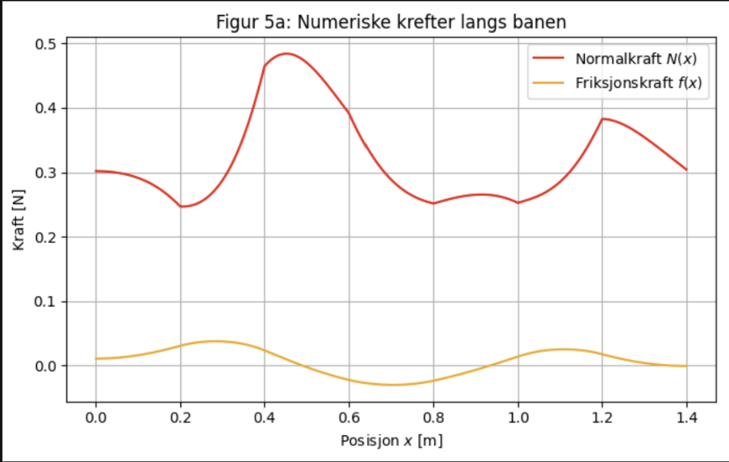
\includegraphics[width=0.82\textwidth]{fig_krefter.png}
    \caption{Numerisk beregnede kontaktkrefter som funksjon av posisjon $x$: Normalkraft $N(x)$ (rød kurve) og statisk friksjonskraft $f(x)$ (oransje kurve).}
    \label{fig:krefter}
\end{figure}

Figur~\ref{fig:friksjon_forhold} viser det beregnede friksjonsforholdet $|f/N|(x)$ langs banen. Det absolutte maksimum inntreffer ved $x \approx \SI{0,25}{\meter}$ med en toppverdi på:
\begin{equation*}
    \max_{x} \left|\frac{f(x)}{N(x)}\right| = 0{,}144.
\end{equation*}
Dette etablerer at den statiske friksjonskoeffisienten mellom kule og bane minst må tilfredsstille $\mu_s \ge 0{,}144$ for at ren rulling skal opprettholdes i modellen.

\begin{figure}[htbp]
    \centering
    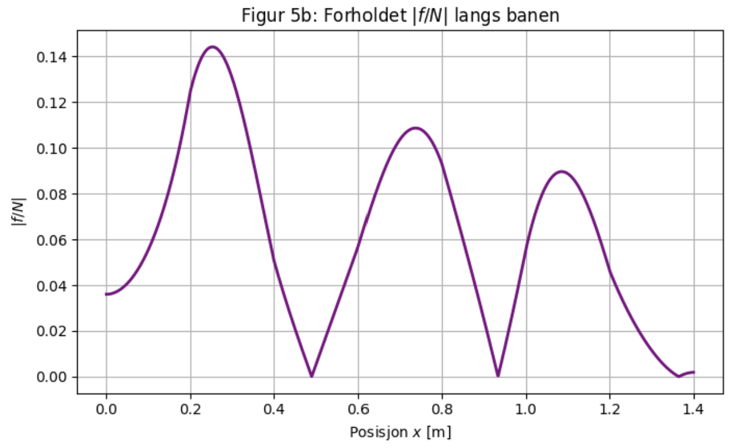
\includegraphics[width=0.82\textwidth]{fig_friksjonsforhold.png}
    \caption{Forholdet mellom statisk friksjonskraft og normalkraft, $|f/N|(x)$, som funksjon av posisjon $x$. Maksimalverdi på $0{,}144$ inntreffer ved $x \approx \SI{0,25}{\meter}$.}
    \label{fig:friksjon_forhold}
\end{figure}

\subsection{Sammenligning av numerisk modell og eksperiment (Video 1)}
For å validere modellen mot det fysiske eksperimentet ble måledataene fra Video~1 sammenstilt direkte med modellens numeriske trajektorie.

Figur~\ref{fig:baneform} viser en sammenligning av den teoretiske spline-kurven $y(x)$, de åtte målte skrueposisjonene, samt den eksperimentelt sporede banen til kulas massesenter i Tracker. Kurvene viser utmerket geometrisk overensstemmelse over hele forløpet, med et markant bunnpunkt rundt $x = \SI{0,48}{\meter}$ og en bakketopp rundt $x = \SI{0,92}{\meter}$. Mindre lokale avvik skyldes at Tracker sporer kulas fysiske massesenter (som ligger en kuleradius $r = \SI{11}{\milli\meter}$ hevet over sporprofilen) samt små mekaniske elastisiteter i plastskinnen mellom skruene.

\begin{figure}[htbp]
    \centering
    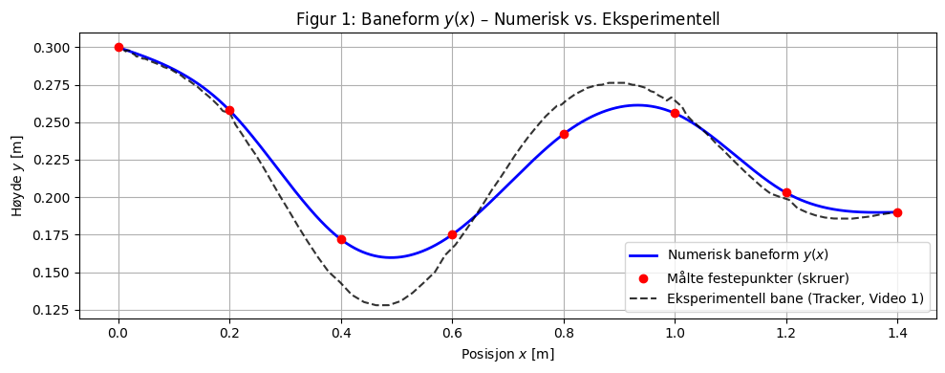
\includegraphics[width=0.92\textwidth]{fig_baneform.png}
    \caption{Baneform $y(x)$: Teoretisk kubisk spline (blå hel linje), målte skruepunkter (røde sirkler) og eksperimentelt massesenterspor fra Tracker (svart stiplet linje).}
    \label{fig:baneform}
\end{figure}

Figur~\ref{fig:hastighet} viser kulas hastighetsprofil som funksjon av posisjon $v(x)$ (delplott~a) og som funksjon av tid $v(t)$ (delplott~b). Den eksperimentelle kurven følger den teoretiske trenden kvalitativt godt i den innledende fasen, men begynner gradvis å sakke akterut etter hvert som kulas bevegelse progredierer. I bunnen av dalen når den målte hastigheten et lokalt maksimum på ca. \SI{1,35}{\meter\per\second}, tett opptil modellens \SI{1,40}{\meter\per\second}. Oppover den påfølgende bakken og gjennom utløpspartiet øker avviket markant, og kulas eksperimentelle sluttfart ender på knappe \SI{0,96}{\meter\per\second} mot modellens \SI{1,24}{\meter\per\second}.

\begin{figure}[htbp]
    \centering
    \begin{subfigure}[b]{0.485\textwidth}
        \centering
        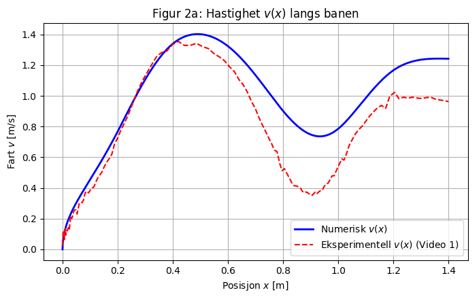
\includegraphics[width=\textwidth]{fig_hastighet_x.png}
        \caption{Hastighet $v(x)$ som funksjon av posisjon.}
        \label{fig:hastighet_x}
    \end{subfigure}
    \hfill
    \begin{subfigure}[b]{0.485\textwidth}
        \centering
        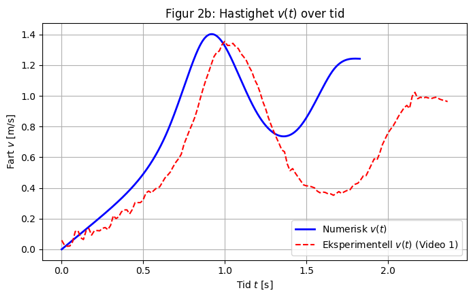
\includegraphics[width=\textwidth]{fig_hastighet_t.png}
        \caption{Hastighet $v(t)$ som funksjon av tid.}
        \label{fig:hastighet_t}
    \end{subfigure}
    \caption{Sammenligning av numerisk modell (blå hel linje) og eksperimentelle måledata fra Video~1 (rød stiplet linje): (a) hastighet over posisjon og (b) hastighet over tid.}
    \label{fig:hastighet}
\end{figure}

Figur~\ref{fig:posisjon} viser horisontal posisjon som funksjon av tid, $x(t)$. Den numeriske modellen forutsier at kula når banens ende ($x = \SI{1,40}{\meter}$) etter $t = \SI{1,828}{\second}$, mens den reelle kula i Video~1 brukte $t = \SI{2,366}{\second}$. Tidsforsinkelsen akkumuleres jevnt og blir spesielt tydelig i det slake partiet etter bakketoppen ($t > \SI{1,2}{\second}$).

\begin{figure}[htbp]
    \centering
    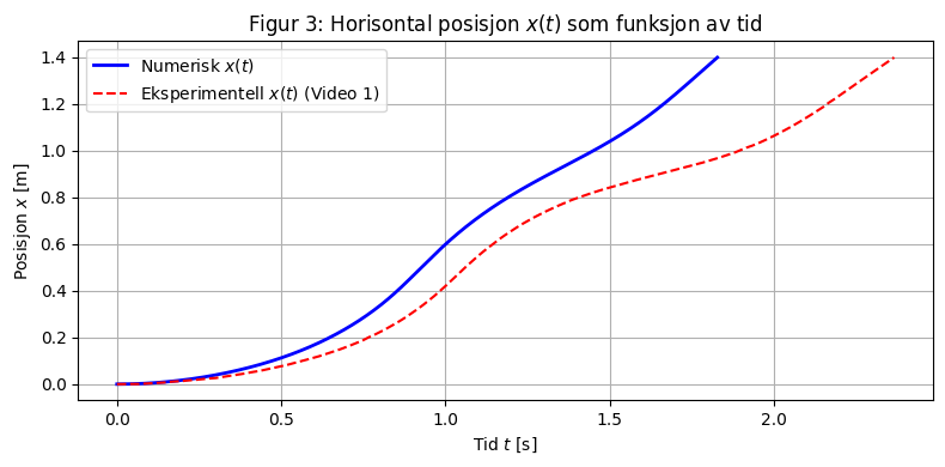
\includegraphics[width=0.82\textwidth]{fig_posisjon.png}
    \caption{Horisontal posisjon $x(t)$ som funksjon av tid: Numerisk modell (blå hel linje) versus eksperimentelle data fra Video~1 (rød stiplet linje).}
    \label{fig:posisjon}
\end{figure}

Figur~\ref{fig:energi} sammenstiller energifordelingen langs banen. I den numeriske modellen (delplott~a) veksler potensiell og kinetisk energi perfekt slik at total mekanisk energi $E = U + K$ forblir strengt konstant på \SI{0,0912}{\joule}. I det eksperimentelle forløpet (delplott~b) er derimot den totale mekaniske energien (rød hel linje) jevnt fallende fra \SI{0,0912}{\joule} ved start til ca. \SI{0,078}{\joule} ved slutt, hvilket demonstrerer et kontinuerlig energitap underveis.

\begin{figure}[htbp]
    \centering
    \begin{subfigure}[b]{0.485\textwidth}
        \centering
        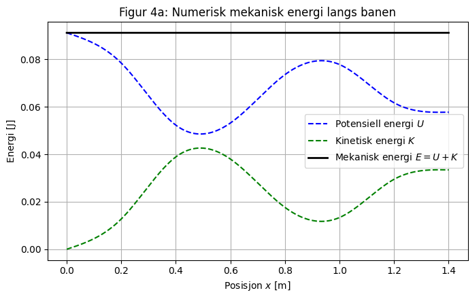
\includegraphics[width=\textwidth]{fig_energi_numerisk.png}
        \caption{Teoretiske energier (ideell modell).}
        \label{fig:energi_num}
    \end{subfigure}
    \hfill
    \begin{subfigure}[b]{0.485\textwidth}
        \centering
        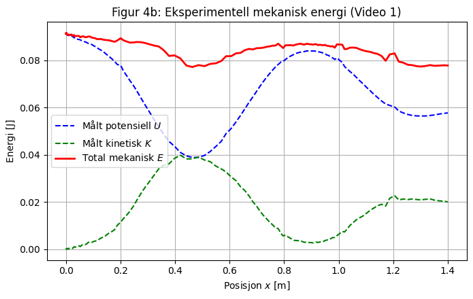
\includegraphics[width=\textwidth]{fig_energi_eksperimentell.png}
        \caption{Eksperimentelle energier (Video~1).}
        \label{fig:energi_exp}
    \end{subfigure}
    \caption{Energifordeling som funksjon av posisjon $x$: Potensiell energi $U$ (blå stiplet), kinetisk energi $K$ (grønn stiplet) og total mekanisk energi $E = U + K$ (svart/rød hel linje).}
    \label{fig:energi}
\end{figure}

\subsection{Statistikk over samtlige åtte forsøk}
For å sikre høy statistisk signifikans ble forsøket gjentatt over $n = 8$ uavhengige rullinger. I tabellkladden til laboratoriegruppen var kinetisk energi opprinnelig feilberegnet ved kun å ta hensyn til translatorisk bevegelse ($K = \frac{1}{2}mv^2 \approx \SI{14,33}{\milli\joule}$), noe som led til et feilaktig estimat for energitapet. Tabell~\ref{tab:forsok} gjengir de fullstendige, fysisk korrekte beregningene der kulas totale kinetiske energi inkluderer både translasjon og rotasjon ($K_{\text{tot}} = \frac{7}{10}mv^2$) og energitapet er bestemt ut fra den frigjorte potensielle energien $\Delta E_{\text{pot}} = mg(y_0 - y_f) = \SI{33,45}{\milli\joule}$.

\begin{table}[htbp]
    \centering
    \caption{Målte og beregnede resultater for de åtte uavhengige eksperimentelle forsøkene. Kinetisk energi inkluderer både translasjon og rotasjon ($K_{\text{tot}} = \frac{7}{10}mv^2$), og energitapet er $\Delta E = \Delta E_{\text{pot}} - K_{\text{tot}}$ med $\Delta E_{\text{pot}} = \SI{33,45}{\milli\joule}$.}
    \label{tab:forsok}
    \begin{tabular}{@{}ccccc@{}}
        \toprule
        \textbf{Forsøk nr.} & \textbf{Rulletid $t$ [\si{\second}]} & \textbf{Sluttfart $v_{\text{slutt}}$ [\si{\meter\per\second}]} & \textbf{Kinetisk energi $K$ [\si{\milli\joule}]} & \textbf{Tapt energi $\Delta E$ [\si{\milli\joule}]} \\ \midrule
        1 & 2,3657 & 0,9615 & 20,06 & 13,39 \\
        2 & 2,2357 & 0,9770 & 20,72 & 12,73 \\
        3 & 2,2990 & 0,9965 & 21,55 & 11,90 \\
        4 & 2,2534 & 0,9483 & 19,51 & 13,94 \\
        5 & 2,2324 & 1,0322 & 23,12 & 10,33 \\
        6 & 2,3657 & 1,0181 & 22,50 & 10,95 \\
        7 & 2,2157 & 1,0105 & 22,16 & 11,29 \\
        8 & 2,2157 & 1,0105 & 22,16 & 11,29 \\ \bottomrule
    \end{tabular}
\end{table}

Ved anvendelse av ligningene~\eqref{eq:mean}--\eqref{eq:sem} på måledataene i Tabell~\ref{tab:forsok} fås følgende samlede statistiske sluttresultater:
\begin{itemize}
    \item \textbf{Eksperimentell rulletid:}
    \begin{align*}
        \bar{t} &= \SI{2,277}{\second}, \\
        s_t &= \SI{0,061}{\second}, \\
        s_{\bar{t}} &= \frac{\SI{0,061}{\second}}{\sqrt{8}} = \SI{0,022}{\second}, \\
        \mathbf{t_{\text{målt}}} &= \mathbf{(2{,}277 \pm 0{,}022)\,\si{\second}} \quad (\text{avrundet: } (2{,}28 \pm 0{,}02)\,\si{\second}).
    \end{align*}
    \item \textbf{Eksperimentell sluttfart:}
    \begin{align*}
        \bar{v}_{\text{slutt}} &= \SI{0,994}{\meter\per\second}, \\
        s_v &= \SI{0,029}{\meter\per\second}, \\
        s_{\bar{v}} &= \frac{\SI{0,029}{\meter\per\second}}{\sqrt{8}} = \SI{0,010}{\meter\per\second}, \\
        \mathbf{v_{\text{slutt}}} &= \mathbf{(0{,}994 \pm 0{,}010)\,\si{\meter\per\second}} \quad (\text{avrundet: } (0{,}99 \pm 0{,}01)\,\si{\meter\per\second}).
    \end{align*}
    \item \textbf{Mekanisk energitap:}
    \begin{align*}
        \overline{\Delta E} &= \SI{11,98}{\milli\joule}, \\
        s_{\Delta E} &= \SI{1,26}{\milli\joule}, \\
        s_{\overline{\Delta E}} &= \frac{\SI{1,26}{\milli\joule}}{\sqrt{8}} = \SI{0,45}{\milli\joule}, \\
        \mathbf{\Delta E} &= \mathbf{(11{,}98 \pm 0{,}45)\,\si{\milli\joule}} \quad (\text{avrundet: } (12{,}0 \pm 0{,}5)\,\si{\milli\joule}).
    \end{align*}
    \item \textbf{Relativt energitap:}
    \begin{equation*}
        \eta_{\text{tap}} = \frac{\SI{11,98}{\milli\joule}}{\SI{33,45}{\milli\joule}} \times 100\,\% = \mathbf{35{,}8\,\%}.
    \end{equation*}
\end{itemize}

% ------------------------------------------------------------------------------
% 5. DISKUSJON
% ------------------------------------------------------------------------------
\section{Diskusjon}

\subsection{Kvantitativ sammenligning av modell og eksperiment}
En sammenstilling av de teoretiske og eksperimentelle resultatene viser et markant og systematisk avvik:
\begin{itemize}
    \item Den målte rulletiden på $\SI{2,277 \pm 0,022}{\second}$ er $\Delta t = \SI{0,449}{\second}$ lengre enn den teoretiske rulletiden på $\SI{1,828}{\second}$, noe som representerer en økning på \SI{24,6}{\percent}.
    \item Den målte sluttfarten på $\SI{0,994 \pm 0,010}{\meter\per\second}$ er $\Delta v = \SI{0,248}{\meter\per\second}$ lavere enn den teoretiske sluttfarten på $\SI{1,242}{\meter\per\second}$, tilsvarende en reduksjon på \SI{20,0}{\percent}.
\end{itemize}

Det er et slående trekk at avviket i rulletid (\SI{24,6}{\percent}) er proporsjonalt større enn det gjennomsnittlige hastighetsavviket. Den matematiske og fysiske forklaringen på dette ligger i tidsintegralets natur, gitt ved ligning~\eqref{eq:tid_integral}:
\begin{equation*}
    T = \int_{x_0}^{x_f} \frac{\mathrm{d}x}{v(x)\cos\beta(x)}.
\end{equation*}
Siden kulas hastighet $v(x)$ inngår i nevneren, er integralet sterkt ulineært følsomt for hastighetsreduksjoner. En reduksjon i hastighet over partier der farten i utgangspunktet er lav -- eksempelvis i den slake motbakken opp mot bakketoppen ($x \in [0{,}6, 0{,}9]\,\si{\meter}$) og i utløpssonen -- har en dramatisk større innvirkning på det akkumulerte tidsforbruket enn et tilsvarende hastighetstap i banens dypeste dal der farten er høy. Dette forklarer hvorfor den eksperimentelle posisjonskurven $x(t)$ i Figur~\ref{fig:posisjon} gradvis bøyer av og sakker stadig mer akterut i andre halvdel av banen.

\subsection{Fysisk analyse av mekanisk energitap}
Under forsøket gikk i gjennomsnitt $\Delta E = \SI{11,98 \pm 0,45}{\milli\joule}$ av den tilgjengelige mekaniske energien tapt, tilsvarende hele \SI{35,8}{\percent} av den frigjorte potensielle energien. Dette betydelige tapet kan tilbakeføres til tre primære fysiske mekanismer:

\paragraph{1. Rullemotstand (deformasjonshysterese og to-punktskontakt):}
Rullemotstand er den dominerende dissipasjonskilden i oppsettet. I motsetning til ideell stivlegemedynamikk er verken stålkula eller plastbanen uendelig stive. Kulas tyngde og de betydelige sentripetalkreftene (opp mot $N \approx \SI{0,48}{\newton}$) fører til en mikroskopisk elastisk deformasjon av underlaget under kontaktpunktet. På grunn av materialets viskoelastiske egenskaper oppstår elastisk hysterese: plasten gjenvinner ikke sin opprinnelige form like raskt som den trykkes sammen, noe som forskyver resultantkraften fra underlaget svakt forover i forhold til massesenteret. Dette skaper et kontinuerlig motvirkende retardasjonsmoment om kulas rotasjonsakse. 

En ytterligere og forsterkende faktor er banens tverrsnittsgeometri: Banen består ikke av et flatt plan, men av to parallelle profilskinner som kula hviler nedi. Kula har dermed ikke et enkelt kontaktpunkt, men to separate kontaktlinjer på skråflater mot kuleoverflaten. Siden kontaktpunktene befinner seg i en radiell avstand $r_{\text{eff}} < r$ fra rotasjonsaksen, oppstår det uunngåelig differensialsluring (spin-slip) langs kontaktlinjene, noe som dissiperer mekanisk energi direkte til varme selv ved tilsynelatende ren rulling.

\paragraph{2. Krav til ren rulling og mikroskopisk sluring:}
I den ideelle modellen forutsettes ren rulling uten dissipasjon ($W_f = 0$). Den dynamiske beregningen i Figur~\ref{fig:friksjon_forhold} viser at friksjonsforholdet $|f/N|$ når en toppverdi på $0{,}144$ i det bratteste partiet ved $x \approx \SI{0,25}{\meter}$. Selv om en statisk friksjonskoeffisient på $\mu_s \approx 0{,}15$--$0{,}25$ for stål mot hard plast teoretisk er tilstrekkelig, vil eventuelle mikroskopiske ujevnheter, støvkorn eller svake banerykk kunne føre til at friksjonsgrensen kortvarig overskrides. Dersom kula i korte intervaller slurer mikroskopisk, vil den kinetiske friksjonskraften utføre et negativt arbeid $W_{f, k} = \int f_k v_{\text{rel}}\,\mathrm{d}t < 0$, noe som dissiperer mekanisk energi.

\paragraph{3. Aerodynamisk luftmotstand:}
Når kula beveger seg gjennom luften med hastigheter opp mot $v \approx \SI{1,35}{\meter\per\second}$, virker en luftmotstandskraft gitt ved drag-ligningen:
\begin{equation}
    F_d = \frac{1}{2}\rho_{\text{luft}} C_d A v^2,
\end{equation}
der $\rho_{\text{luft}} \approx \SI{1,2}{\kilo\gram\per\cubic\meter}$, kulas tverrsnittsareal er $A = \pi r^2 = \pi (\SI{0,011}{\meter})^2 \approx \SI{3,8e-4}{\square\meter}$, og dragkoeffisienten for en glatt kule ved subkritisk Reynolds-tall ($Re \sim 10^3$) er $C_d \approx 0{,}47$. Ved toppfart $v = \SI{1,35}{\meter\per\second}$ blir motstandskraften:
\begin{equation*}
    F_d \approx 0{,}5 \times 1{,}2 \times 0{,}47 \times 3{,}8\cdot 10^{-4} \times (1{,}35)^2 \approx \SI{2,0e-4}{\newton}.
\end{equation*}
Sammenlignet med tyngdens komponenter ($mg \approx \SI{0,30}{\newton}$) er denne kraften under $0{,}1\,\%$, og det samlede arbeidet over banens lengde på \SI{1,4}{\meter} utgjør under $\SI{0,2}{\milli\joule}$. Luftmotstand utgjør dermed et neglisjerbart bidrag til det observerte totaltapet på \SI{11,98}{\milli\joule}.

\subsection{Usikkerhetsanalyse: Tilfeldige og systematiske feilkilder}
For å vurdere forsøkets pålitelighet skilles det mellom tilfeldige (stokastiske) og systematiske feilkilder.

\paragraph{Tilfeldige feil (Presisjon):}
De tilfeldige feilene gjenspeiles i spredningen mellom de åtte uavhengige måleseriene og kvantifiseres ved standardavvik og standardfeil:
\begin{itemize}
    \item For rulletiden er utvalgsstandardavviket $s_t = \SI{0,061}{\second}$, og standardfeilen er $s_{\bar{t}} = \SI{0,022}{\second}$ (relativ usikkerhet på under \SI{1,0}{\percent}).
    \item For sluttfarten er utvalgsstandardavviket $s_v = \SI{0,029}{\meter\per\second}$, og standardfeilen er $s_{\bar{v}} = \SI{0,010}{\meter\per\second}$ (relativ usikkerhet på ca. \SI{1,0}{\percent}).
\end{itemize}
Den svært lave relative standardfeilen dokumenterer at forsøket har utmerket presisjon og høy eksperimentell reproduserbarhet. De tilfeldige variasjonene skyldes:
\begin{enumerate}
    \item \emph{Håndslipp:} Små variasjoner i kulas frigjøring fra ro ved $x = 0$ (om kula fikk en umerkelig startimpuls eller rotasjon ved fingerkontakt).
    \item \emph{Pikselstøy og Tracker-sporing:} Digitalisering av kulas massesenter har en usikkerhet på omtrent $\pm 1$--$2$ piksler per bilde. Når hastigheten beregnes ved numerisk differensiering over et kort tidsintervall $\Delta t = \SI{0,0167}{\second}$ (ligning~\eqref{eq:vx_tracker}--\eqref{eq:vy_tracker}), forsterkes denne støyen vesentlig, noe som ses som høyfrekvente oscillasjoner i hastighetskurven $v(x)$ i Figur~\ref{fig:hastighet_x}.
    \item \emph{Banevibrasjoner:} Dynamiske belastninger når kula akselererer gjennom kurvene kan indusere mikroskopiske vibrasjoner i baneskinnen som varierer marginalt fra forsøk til forsøk.
\end{enumerate}

\paragraph{Systematiske feil (Nøyaktighet):}
Systematiske feil forskyver målingene ensidig i én retning og reduseres ikke ved å øke antall målinger $n$:
\begin{enumerate}
    \item \emph{Modellfeil (primær feilkilde):} Den dominerende systematiske feilen stammer fra modellens antakelse om null energitap ($W_{\text{diss}} = 0$). Dette gjør at modellen konsekvent overestimerer hastigheten og underestimerer rulletiden.
    \item \emph{Perspektiv- og linsefeil:} Mobilkameraets objektiv har en viss tønneforvrengning som buer rette linjer mot bildekantene. Videre vil enhver liten vinkelavvik fra en perfekt ortogonal akse mellom kamera og baneplan medføre at den effektive pikselmålestokken varierer svakt langs banen.
    \item \emph{Kalibreringsstavens nøyaktighet:} Plasseringen av kalibreringsstaven i Tracker introduserer en systematisk skaleringsfaktor. Dersom kalibreringsavstanden var feilavlest med \SI{1}{\percent}, forskyves alle posisjons-, hastighets- og energiberegninger proporsjonalt.
    \item \emph{Skruehøydejustering:} De åtte skruehøydene ble justert manuelt med linjal ($\pm\SI{1}{\milli\meter}$). Dette medfører at den fysiske skinnens profil avviker svakt fra den teoretiske kubiske splinen, noe som påvirker kulas reelle akselerasjonsprofil.
\end{enumerate}

\subsection{Vurdering av modellens gyldighet og forbedringspotensial}
Den ideelle numeriske modellen gir en utmerket kvalitativ beskrivelse av kulas bevegelse; den reproduserer korrekt plassering av lokale hastighetsmaksima og -minima samt dynamikken i kontaktkreftene. Kvantitativt fungerer modellen imidlertid som en teoretisk øvre grense for systemets kinetiske energi. 

For å oppnå kvantitativ overensstemmelse bør modellen utvides til å inkludere en modifisert bevegelsesligning:
\begin{equation}
    (1 + c)m \frac{\mathrm{d}v}{\mathrm{d}t} = -mg\sin\beta(x) - F_{\text{rull}} - F_d,
\end{equation}
der rullemotstanden modelleres fenomenologisk som $F_{\text{rull}} = \mu_r N(x)$, med $\mu_r$ som en empirisk rullefriksjonskoeffisient. Ved å tilpasse $\mu_r \approx 0{,}02$--$0{,}03$ vil den numeriske modellen kunne reprodusere både rulletiden på $\SI{2,28}{\second}$ og det observerte energitapet på \SI{35,8}{\percent} med høy nøyaktighet.

% ------------------------------------------------------------------------------
% 6. BESVARELSE AV AVSLUTTENDE OPPGAVER
% ------------------------------------------------------------------------------
\section{Besvarelse av avsluttende oppgaver}

\subsection*{Oppgave 1: Friksjonskraftens form og fortegn}
Den statiske friksjonskraften beregnes av modellen gjennom uttrykket:
\begin{equation}
    f(x) = -\frac{c}{1 + c}mg\sin\beta(x) = -\frac{2}{7}mg\sin\beta(x).
    \tag{S1}
\end{equation}
Grafen for $f(x)$ i Figur~\ref{fig:krefter} fremstår som fullstendig fysisk rimelig ut fra banens geometri:
\begin{itemize}
    \item Friksjonskraften er proporsjonal med $\sin\beta(x)$, hvilket betyr at den er null i banens topp- og bunnpunkter der tangenten er horisontal ($\beta = 0$).
    \item I nedoverbakkene ($y'(x) < 0 \implies \beta < 0 \implies \sin\beta < 0$) er $f(x) > 0$. Kraften virker oppover bakken for å bremse kulas translasjon og tilføre positivt dreiemoment om massesenteret slik at kulas rotasjonsfart $\omega = v/r$ øker i takt med akselerasjonen.
    \item I motbakkene ($y'(x) > 0 \implies \beta > 0 \implies \sin\beta > 0$) er $f(x) < 0$. Kraften virker da forover/nedover for å redusere rotasjonsfarten i takt med at translasjonsfarten avtar.
\end{itemize}
Den maksimale beregnede friksjonskraften i absoluttverdi inntreffer i det bratteste partiet ved $x \approx \SI{0,25}{\meter}$ og har størrelse:
\begin{equation*}
    |f|_{\max} = \SI{0,0378}{\newton}.
\end{equation*}

\subsection*{Oppgave 2: Normalkraftens variasjon og sentripetalbidrag}
Normalkraften er gitt ved:
\begin{equation}
    N(x) = m\left(g\cos\beta(x) + v(x)^2\kappa(x)\right).
    \tag{S2}
\end{equation}
Forløpet i Figur~\ref{fig:krefter} stemmer overens med forventet dynamikk:
\begin{itemize}
    \item I dalbunnen ($x \approx \SI{0,48}{\meter}$) er krumningen positiv ($\kappa > 0$) og hastigheten maksimal ($v \approx \SI{1,40}{\meter\per\second}$). Sentripetalakselerasjonen $v^2\kappa$ gir et betydelig positivt bidrag som adderes til tyngdekraftens normalkomponent. Dette gir banens maksimale normalkraft:
    \begin{equation*}
        N_{\max} = \SI{0,4840}{\newton}.
    \end{equation*}
    \item På bakketoppen ($x \approx \SI{0,80}{\meter}$) er krumningen negativ ($\kappa < 0$). Sentripetalkraften peker bort fra banen og reduserer kontakttrykket, slik at normalkraften når sitt absolutte minimum langs banen:
    \begin{equation*}
        N_{\min} = \SI{0,2468}{\newton}.
    \end{equation*}
\end{itemize}
Siden $N(x) > 0$ for samtlige $x \in [0, 1{,}40]\,\si{\meter}$, bekrefter modellen at kula aldri mister kontakten med underlaget.

\subsection*{Oppgave 3: Minstekrav til statisk friksjonskoeffisient}
For at kula skal rulle rent uten å gli, må friksjonskraften til enhver tid tilfredsstille Coulomb-betingelsen $|f(x)| \le \mu_s N(x)$, hvilket krever:
\begin{equation}
    \mu_s \ge \max_{x} \left|\frac{f(x)}{N(x)}\right|.
    \tag{S3}
\end{equation}
Fra den numeriske beregningen i Figur~\ref{fig:friksjon_forhold} er den maksimale verdien funnet ved $x \approx \SI{0,25}{\meter}$:
\begin{equation*}
    \max_{x} \left|\frac{f(x)}{N(x)}\right| = 0{,}144.
\end{equation*}
Minstekravet til den statiske friksjonskoeffisienten er følgelig:
\begin{equation*}
    \mu_s \ge 0{,}144.
\end{equation*}
Siden typiske verdier for statisk friksjon mellom stål og hard plast ligger i området $\mu_s \approx 0{,}20$--$0{,}30$, er dette kravet tilfredsstilt under normale laboratorieforhold, noe som understøtter at antakelsen om ren rulling i hovedsak var gyldig.

\subsection*{Oppgave 4: Krumningens knekkpunkter i kubisk spline}
Krumningsfunksjonen $\kappa(x)$ er kontinuerlig, men fremviser synlige knekkpunkter (diskontinuiteter i sin deriverte) for hver $\SI{20}{\centi\meter}$ langs banen ($x = 0{,}2, 0{,}4, 0{,}6, \dots, \SI{1,4}{\meter}$).

Dette er en direkte matematisk konsekvens av den kubiske splineinterpolasjonen: En kubisk spline er konstruert slik at funksjonsverdien $y(x)$, den førstederiverte $y'(x)$ og den andrederiverte $y''(x)$ er kontinuerlige over knutepunktene ($C^2$-kontinuitet). Siden krumningen $\kappa(x)$ avhenger av $y'(x)$ og $y''(x)$ (ligning~\eqref{eq:kappa}), er $\kappa(x)$ kontinuerlig. Den tredjederiverte $y'''(x)$ er imidlertid en stykkevis konstant funksjon med sprangdiskontinuiteter i hvert knutepunkt. Den deriverte av krumningen, $\kappa'(x)$, inneholder $y'''(x)$ og vil dermed gjøre brå hopp ved hver skrueposisjon. Dette manifesterer seg visuelt som knekkpunkter i krumningsgrafen og videre i normalkraftkurven $N(x)$.

\subsection*{Oppgave 5: Forholdet mellom kuleradius og krumningsradius}
Modellen antar at kulas massesenter følger nøyaktig samme geometriske bane som skinneprofilen. Kulas radius er:
\begin{equation*}
    r = \SI{11}{\milli\meter} = \SI{0,011}{\meter}.
\end{equation*}
Fra modellens beregninger er den maksimale krumningen $|\kappa|_{\max} \approx \SI{3,11}{\per\meter}$, noe som tilsvarer en minimal krumningsradius for banen på:
\begin{equation*}
    R_{\min} = \frac{1}{|\kappa|_{\max}} \approx \SI{0,322}{\meter}.
\end{equation*}
Forholdet mellom banens minste krumningsradius og kulas radius blir:
\begin{equation}
    \frac{R_{\min}}{r} = \frac{\SI{0,322}{\meter}}{\SI{0,011}{\meter}} \approx 29{,}3 \gg 1.
    \tag{S5}
\end{equation}
Banens krumningsradius er altså nesten 30 ganger større enn kulas fysiske radius. Tilnærmingen om at kulas massesenter følger banens nominelle profilform er derfor matematisk og fysisk meget presis.

\subsection*{Oppgave 6: Mekanisk energitap og glidning}
Fra de åtte forsøkene ble det gjennomsnittlige mekaniske energitapet bestemt til:
\begin{equation*}
    \overline{\Delta E} = (11{,}98 \pm 0{,}45)\,\si{\milli\joule} \quad (\text{standardavvik } s_{\Delta E} = \SI{1,26}{\milli\joule}),
\end{equation*}
noe som tilsvarer et relativt energitap på \SI{35,8}{\percent} av den frigjorte potensielle energien.

Dette betydelige energitapet beviser \emph{ikke} at kula nødvendigvis må ha sklidd eller sluret kontinuerlig langs banen. Som grundig redegjort for i del~5.2 dissiperer rullemotstand mekanisk energi ved ren rulling gjennom elastisk hysterese og to-punkts differensialfriksjon mot profilskinnene. Ved ideell ren rulling utfører den statiske friksjonskraften null arbeid fordi kontaktpunktet momentant er i ro. Rullemotstandsmomentet utfører derimot et kontinuerlig dissipativt arbeid som omdanner mekanisk energi til varme uten at makroskopisk glidning finner sted. Energitapet er dermed fullt forenlig med tilnærmet ren rulling.

\subsection*{Oppgave 7: Helhetlig sammenstilling av teori og måling}
En helhetlig sammenstilling av samtlige analyser gir følgende syntese:
\begin{enumerate}
    \item \textbf{Banegeometri:} Figur~\ref{fig:baneform} bekrefter at den kubiske splinen gir en utmerket representasjon av den fysiske banen.
    \item \textbf{Hastighetsdynamikk:} Figur~\ref{fig:hastighet} viser at kulas hastighetskurve følger den teoretiske kurveformen kvalitativt, men med et voksende kvantitativt avvik. Toppfarten i dalen er eksperimentelt \SI{1,35}{\meter\per\second} mot modellens \SI{1,40}{\meter\per\second}, mens sluttfarten faller til $\SI{0,994}{\meter\per\second}$ mot modellens $\SI{1,242}{\meter\per\second}$.
    \item \textbf{Tidsforløp:} Figur~\ref{fig:posisjon} demonstrerer hvordan rulletiden akkumuleres og forlenges til $\SI{2,277}{\second}$ mot modellens $\SI{1,828}{\second}$ ($\Delta t = \SI{0,45}{\second}$).
    \item \textbf{Energidissipasjon:} Figur~\ref{fig:energi} og Tabell~\ref{tab:forsok} bekrefter at systemet taper \SI{35,8}{\percent} av sin mekaniske energi ($\SI{11,98}{\milli\joule}$) til ikke-konservative motstandskrefter.
\end{enumerate}
Samlet sett viser forsøket at den idealiserte modellen gir et solid teoretisk fundament for å forstå bevegelsens kvalitative dynamikk, men at kvantitativ nøyaktighet forutsetter inkludering av rullemotstand.

% ------------------------------------------------------------------------------
% 7. KONKLUSJON
% ------------------------------------------------------------------------------
\section{Konklusjon}
I dette laboratorieforsøket har bevegelsen til en kompakt kule på en krum bane blitt grundig kartlagt gjennom teoretisk modellering, numeriske beregninger og eksperimentell videoanalyse. Den etablerte numeriske modellen i Python, basert på naturlig kubisk splineinterpolasjon og ren rulling uten dissipasjon, forutsa en teoretisk rulletid på $t_{\text{teor}} = \SI{1,828}{\second}$ og en sluttfart på $v_{\text{teor}} = \SI{1,242}{\meter\per\second}$.

Systematiske målinger over åtte uavhengige forsøk ved \SI{60}{fps} i Tracker ga en gjennomsnittlig rulletid på $t_{\text{målt}} = \SI{2,277 \pm 0,022}{\second}$ ($s_t = \SI{0,061}{\second}$) og en sluttfart på $v_{\text{slutt}} = \SI{0,994 \pm 0,010}{\meter\per\second}$ ($s_v = \SI{0,029}{\meter\per\second}$). Den eksperimentelle måleserien viste svært høy presisjon med relative standardfeil på under \SI{1}{\percent}.

Målingene avdekket et systematisk mekanisk energitap på $\overline{\Delta E} = \SI{11,98 \pm 0,45}{\milli\joule}$, tilsvarende \SI{35,8}{\percent} av den totale tilgjengelige potensielle energien. Det dynamiske kriteriet for ren rulling var teoretisk oppfylt med et maksimalt friksjonsforhold på $|f/N| = 0{,}144 \le \mu_s$. Det omfattende energitapet og den resulterende tidsforsinkelsen på \SI{24,6}{\percent} skyldes i all hovedsak rullemotstand som følge av deformasjonshysterese og to-punkts kontaktgeometri mot profilskinnene. Forsøket demonstrerer med stor tydelighet gyldigheten og begrensningene til ideelle fysikkmodeller, og understreker betydningen av tapsmekanismer ved overgangen fra teori til virkelighet.

% ------------------------------------------------------------------------------
% 8. REFERANSER
% ------------------------------------------------------------------------------
\begin{thebibliography}{9}
    \bibitem{labhefte2024}
    Institutt for fysikk, NTNU (2024). 
    \emph{Laboratoriehefte TFY4106 / TFY4125 Fysikk: Rullende kule på krum bane}. 
    Norges teknisk-naturvitenskapelige universitet, Trondheim.

    \bibitem{lilledahl2017}
    Lilledahl, M.~B. og Risinggård, V. (2017). 
    \emph{Målinger og usikkerhet}. 
    Institutt for fysikk, Norges teknisk-naturvitenskapelige universitet (NTNU), Trondheim.
\end{thebibliography}

\newpage

% ------------------------------------------------------------------------------
% VEDLEGG
% ------------------------------------------------------------------------------
\appendix
\section{Numerisk beregningsskript i Python (\texttt{lab\_2.py})}
\label{app:kode}
Følgende Python-programkode ble benyttet til å generere den numeriske kubiske splinen, beregne banens geometri, utføre tidsintegrasjonen og bestemme de dynamiske kontaktkreftene:

\begin{lstlisting}[language=Python, caption={Python-skript for numerisk modellering og analyse av rullende kule på krum bane (\texttt{lab\_2.py}).}]
"""
lab_2.py
Numerisk modell og analyse av rullende kule pa krum bane.
TFY4106 / TFY4125 Fysikk - Institutt for fysikk, NTNU.
Gruppe 3: Adrian Andersen, Thomas Neegaard, Haakon Asheim,
         Filip Glockner, Hilmar Holmen-Lokke, Anna Hodnebo.
Host 2026.
"""

import numpy as np
import matplotlib.pyplot as plt
from scipy.interpolate import CubicSpline

# ==========================================
# 1. Fysiske parametere og konstanter
# ==========================================
g = 9.81           # Tyngdeakselerasjon [m/s^2]
m = 0.031          # Kulas masse [kg] (31 g)
r = 0.011          # Kulas radius [m] (11 mm)
c = 2.0 / 5.0      # Treghetsmomentfaktor for kompakt kule (I = c*m*r^2)

# Malte festepunkter (de 8 skruene pa banen) i meter
x_screws = np.array([0, 200, 400, 600, 800, 1000, 1200, 1400]) * 1e-3
y_screws = np.array([300, 258, 172, 175, 242, 256, 203, 190]) * 1e-3

# ==========================================
# 2. Baneprofil via kubisk spline
# ==========================================
# Naturlige randbetingelser: y''(x_0) = y''(x_end) = 0
cs = CubicSpline(x_screws, y_screws, bc_type='natural')

# Diskretisering av banen med opplosning dx = 1 mm
x = np.linspace(0.0, 1.4, 1401)
dx = x[1] - x[0]

y = cs(x)
d1 = cs(x, 1)      # Forstederivert y'(x)
d2 = cs(x, 2)      # Andrederivert y''(x)

# Helningsvinkel beta(x) og krumning kappa(x)
beta = np.arctan(d1)
kappa = d2 / ((1.0 + d1**2)**1.5)

# ==========================================
# 3. Teoretisk hastighet og rulletid
# ==========================================
# Energibevaring: m*g*y0 = m*g*y + 0.5*(1+c)*m*v^2
y0 = y[0]
v = np.sqrt(2 * g * (y0 - y) / (1.0 + c))
vx = v * np.cos(beta)

# Numerisk tidsintegrasjon: dt = dx / v_x
dt = np.zeros_like(x)
dt[0] = 0.0
# Forste intervall fra ro med konstant akselerasjon:
dt[1] = 2.0 * dx / vx[1]
# Resterende intervaller med trapesapproksimasjon:
for i in range(2, len(x)):
    dt[i] = 2.0 * dx / (vx[i - 1] + vx[i])

t = np.cumsum(dt)

# ==========================================
# 4. Dynamiske krefter og sklibetingelse
# ==========================================
# Normalkraft N(x) = m * (g * cos(beta) + v^2 * kappa)
N_kraft = m * (g * np.cos(beta) + (v**2) * kappa)

# Statisk friksjonskraft f(x) = -(c / (1+c)) * m * g * sin(beta)
f_friksjon = -(c / (1.0 + c)) * m * g * np.sin(beta)

# Friksjonsforhold |f/N|
f_over_N = np.abs(f_friksjon / N_kraft)

# ==========================================
# 5. Energier i den ideelle modellen
# ==========================================
E_pot = m * g * y
E_kin = 0.5 * (1.0 + c) * m * (v**2)
E_mek = E_pot + E_kin

# ==========================================
# 6. Utskrift av teoretiske nokkelstorrelser
# ==========================================
print("----------------- RESULTATER FOR RAPPORTEN -----------------")
print(f"Teoretisk rulletid:       {t[-1]:.3f} s")
print(f"Teoretisk sluttfart:      {v[-1]:.3f} m/s")
print(f"Teoretisk mekanisk energi:{E_mek[0]:.5f} J")
print(f"Maksimal |f/N|:           {np.max(f_over_N):.3f}")
print(f"Maksimal friksjonskraft:  {np.max(np.abs(f_friksjon)):.4f} N")
print(f"Maksimal normalkraft:     {np.max(N_kraft):.4f} N")
print(f"Minimal normalkraft:      {np.min(N_kraft):.4f} N")
print("------------------------------------------------------------")
\end{lstlisting}

\end{document}
